%%%%%%%%%%%%%%%%%%%%%%%%%%%%%%%%%%%%%%%%%%%%%%%%%%%
%%         LegoNXT in  Physical Etoys            %%
%%                                               %%
%%                GIRA 2011                      %%
%% Planète Sciences 20011 for the Latex version) %%
%%%%%%%%%%%%%%%%%%%%%%%%%%%%%%%%%%%%%%%%%%%%%%%%%%%

%% Authors: Ricardo Moran

\documentclass[english]{etoys-guide}

\usepackage{babel}
\usepackage{etoys}


%%%%%%%%%%%%%%%%%%%%%%%%%%%%%%%%%%%%%%%%%%%%%%%%%%%%%%%%%%%%%%%%%%%%%%%%%%%%%%%
%%                           Glossary                                        %%
%%%%%%%%%%%%%%%%%%%%%%%%%%%%%%%%%%%%%%%%%%%%%%%%%%%%%%%%%%%%%%%%%%%%%%%%%%%%%%%

\newglossaryentry{halo}
		{name={halo}, 
		description={The \emph{halo} is the set of icons that surround an object when we \rc on it}}
\newglossaryentry{script}
		{name={script}, 
		description={The \emph{scripts} are the small programs attached to each object. You can see all scripts for a given object from its \keyword{viewer}, in the \important{scripts} category}
		plural={scripts}}
\newglossaryentry{viewer}
		{name={viewer}, 
		description={The \emph{viewer} of an object is the object-specif flap that holds all the tiles enabling programming. You can open it up with \icon[eye]{eye} in the objects's \keyword{halo}. The viewer is divided in \emph{Categories} that organize the tiles}}
\newglossaryentry{heading}
		{name={heading}, 
		description={An object's \emph{heading} is its orientation relative to its \emph{forward direction}, in degrees. A null heading means the object is oriented towards its ``forward direction''. To change the heading, you can use \icon[rotate]{rotate}. The green arrow that appears in the centre of the object indicates the forward direction. You can change it by drag and drop \important{while maintaining the Shift key pressed}}}
\newglossaryentry{parameter}
		{name={parameter}, 
		description={A parameter of a function (or a script) is an option given to the function that we can modify outside of the function}}
\newglossaryentry{world}
		{name={World}, 
		description={The \emph{World} is the \appName desktop as a whole. It is actually an object, similar to the other ones: you can display its \keyword{halo}, open up its \keyword{viewer}, attach \keywordpl{script} to it...}}
\newglossaryentry{photoresistor}
		{name={photoresistor}, 
		description={A \emph{photoresistor} is a small \keyword{passive sensor} whose resistance increases when the ambient light decreases}}
\newglossaryentry{passive sensor}
		{name={passive sensor}, 
		description={A \emph{passive sensor} is a sensor that does not require an external power source to operate. For instance, the \keyword{photoresistor} or the thermistor}}
\newglossaryentry{variable}
		{name={variable}, 
		plural={variables}, 
		description={A variable is a \emph{label} you can create in an object, that \emph{references} another object, or a text, a numerical value,... It mainly allows us to use or manipulate this referenced object in a script}}
%%%%%%%%%%%%%%%%%%%%%%%%%%%%%%%%%%%%%%%%%%%%%%%%%%%%%%%%%%%%%%%%%%%%%%%%%%%%%%%


\def\appName{Physical~Etoys~}

%%%%%%%%%%%%%%%%%%%%%%%%%%%%%%%%%%%%%%%%%%%%%%%%%%%%%%%%%%%%%%%%%%%%%%%%%%%%%%%%%
%%%%%%%%%%%%%%%%%%%%%%%%%%%%%%%%%%%%%%%%%%%%%%%%%%%%%%%%%%%%%%%%%%%%%%%%%%%%%%%%%

\title{
	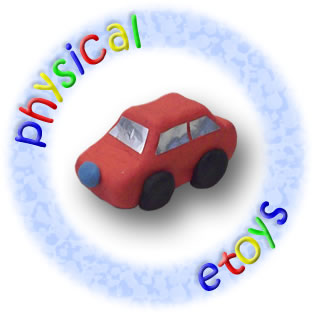
\includegraphics[width=8cm]{../../shared/images/physical_etoys_logo.jpg}\\
	\vfill
	%
\includegraphics[width=5cm]{minibot.png}
	\vspace{3em}
	\LARGE{\textbf{\appName~and the LegoNXT}}\\[1cm]
	\large{Step by step into interfacing LegoNXT with \appName}\\[1cm]
	\vfill
}

\author{
GIRA
}

%%%%%%%%%%%%%%%%%%%%%%%%%%%%%%%%%%%%%%%%%%%%%%%%%%%%%%%%%%%%%%%%%%%%%%%%%%%%%%%%%
%%%%%%%%%%%%%%%%%%%%%%%%%%%%%%%%%%%%%%%%%%%%%%%%%%%%%%%%%%%%%%%%%%%%%%%%%%%%%%%%%
\begin{document}

% If a PDF file called 'cover.pdf' exists, use it as cover.
\IfFileExists{cover.pdf}{
\includepdf[pages=-, fitpaper]{cover.pdf}
\thispagestyle{empty}
\cleardoublepage
}

\maketitle

\cleardoublepage
\tableofcontents
\cleardoublepage


\appName is a software Project which let us control, in real time, Lego
Mindstorms Nxt’s Robots using a Bluetooth connection. SqueakNxt is a module of
the \appName software.

In this tutorial we will introduce \appName and, step by step, show its basic
characteristics. 


%%%%%%%%%%%%%%%%%%%%%%%%%%%%%%%%%%%%%%%%%%%%%%%%%%%%%%%%%%%%%%%%%%%%%%%%%%%%%%%%%
\section{Installation}

\subsection{Necessary tools}

\begin{itemize}
	\item A Lego Mindstorms NXT robot,
	\item A Bluetooth device (like a laptop with Bluetooth),
	\item \appName software.
\end{itemize}

\subsection{Configuring Bluetooth} 

The first step is to configure the Bluetooth in order to connect the robot with
the computer.

Turn the robot on by pressing the orange button.

\screenshot{1.png}

Insert the Bluetooth device into the computer. Then we doubleclick the
Bluetooth icon which appears on the taskbar.

\screenshot{2.png}


The Bluetooth device window will appear. Then we click on the “add” button.


\screenshot{3.png}



We choose “My device is set up and ready to be found”. Then we select the
device we want to connect and click on next. We choose “let me choose my own
passkey” and then we type a new one. Eg.: 1234


\screenshot{4.png}

We enter the chosen passkey for the robot and we confirm it by pressing the
orange button. 


\screenshot{5.png}

The COM ports will be assigned automatically (not necessarily six and seven).
The port that we are going to use is the output port so we have to remember its
number. 


\screenshot{6.png}

Now we are ready to connect the robot with \appName. 

\subsection{Connection to \appName}

First and foremost, inside \appName, we have to get a “Nxt brick”. This is a
graphical object that represents the computer of the real robot. In order to
obtain it we have to open the supplies’ flap.


\screenshot{7.png}

The supplies’ flap contains the most used objects.  As long as we use the
system we are going to learn more things about them. The one that interests us
is the “Object catalog”.


\screenshot{8.png}

Now we have to drop the object catalog on the world. 


\screenshot{9.png}

The object catalog is like a box that contains the entire objects that we can
use. It is ordered by categories but we can arrange the objects alphabetically.
Apart from that we can look for a particular one. Now we have to choose the
Lego Nxt category. 


\screenshot{10.png}

Then we have to drag the “Nxt Brick” etoy and place it on the world.


\screenshot{11.png}


Once we have the “Nxt brick” we have to choose the same number of port that the
Bluetooth output port (we can change the number by clicking on the triangled
buttons) and then we have to confirm by clicking on the orange button. The
robot would play a confirmation sound and the “Nxt Brick” would be like this:


\screenshot{12.png}


\section{First experiment: Playing a sound}

The first action that we can do is playing a sound inside the robot. 

We have to open its viewer by making right-click on the Nxt Brick to open the
halo. The halo is a set of buttons which surround the object and let the user
modify, move, delete and maximize it.

\screenshot{13.png}

Next we click on the viewer icon (light blue) to make it appear. 

\screenshot{14.png}


The viewer is a flap where we can not only see and modify the object’s
properties on the screen but also create scripts for them to perform actions
like moving on the screen. The properties and the actions are represented as
tiles.

\screenshot{15.png}

In this category (lego nxt – other stuff) we can see all the tiles that can be
used to communicate with the robot. The instruction that we are going to use
now is “play tone”. If we change the “5” parameter for a higher number, e.g.
2000, and then we run the tile (by clicking on the yellow button which has an
exclamation character) we will listen to a high-pitched sound. 

\section{Changing the motor speed}

Now that the first exercise has been done we can do more interesting things
such as modifying the motor speed.  First we have to plug a motor on the
robot’s port A. In addition, we have to “plug” a motor in the computer. So we
have to look for a NxtMotor in the object catalog, then we drag and drop it on
the port A of the “Nxt brick”.


\screenshot{16.png}


A cable may appear and connect the motor with the “Nxt brick”. Now we have to
open the motor’s viewer in order to access its instructions.



\screenshot{17.png}


\screenshot{18.png}


We are interested in the “power” property. With this property we can change or
read the current speed of the motor (now it is zero because the motor is not
moving).


\screenshot{19.png}


If we modify the power value from 0 to 100 we will see that the motor moves for
an instant but then it stops due to the “automatic brake” property. When its
value is true and the motor does not receive a new power value the motor stops
automatically.

If we want the motor to go on with the same speed we have to change the value
of the “automatic brake” property to false. Another possibility is to create a
new script which sends the new speed to the motor regularly. The best choice is
creating a new script. 

We drag the “power” property from the arrow (it means an assignation) and then
we drop it on outside. 

\screenshot{20.png}

By doing this a new script called “script1” will be created. This script only
has one instruction: setting up the motor with no velocity. In order to move
the motor we have to assign it a new value.


\screenshot{21.png}

We have to change the value to 100 and then we run the script by clicking on
the button which is similar to a clock.


\screenshot{22.png}

\screenshot{23.png}


The clock will become blue and the state will change to “ticking”. This means
that the script is running and the motor may be working at max speed. If we
click again on the clock, the script will stop and, after a few seconds, the
motor will stop also (unless the “automatic brake property” is false).

This script will leave the motor functioning at constant speed. It will be
interesting if we can modify the speed without changing the script “code”. In
order to do this we can use a “Slider” which is an object that we can find in
the objects catalog under the “Basic” category. 


\screenshot{24.png}

The slider let us choose a number by dragging a bar. If we open the slider’s
viewer we will see a property called “numeric value” ranging from 0 to 1
depending on the location of the bar (down=0 and up=1).



\screenshot{25.png}

We need to use this property to control the motor’s speed. We drag the property
from its name (not from the arrow because we want only to return the value that
the slider has) and then we replace the 100 with the tile.

\screenshot{26.png}


With this change the motor will stop because the “numeric value” at this moment
has a little value which is not longer than 1. 

To move the motor considerably we have to assign it speeds ranging from 0 to
100. So we need to multiply the value of “numeric value” by 100. In order to do
this we have to click on the little arrow which is on the right-hand side of
“numeric value” (when the cursor is over the arrow it will become bigger.  


\screenshot{27.png}

\screenshot{28.png}



This let us make operations with the slider’s value. We need to replace the “1”
with “100” and the addition with a multiplication.   


\screenshot{29.png}

\screenshot{30.png}


Now by moving the slider’s bar we can change the motor’s speed. 

\section{Reading a sensor’s value}

The last but not least activity that we can do is reading sensor’s values.
First we have to plug a light sensor on the robot’s port 1. Now, in the
computer, we have to “plug” a “Nxt Light sensor” in port 1 of the “Nxt brick”.
We can click on port 1 of the “Nxt brick” and then choose the “Nxt Light
sensor”. It will look like this: 


\screenshot{31.png}


Now we open the viewer of the “Nxt Light Sensor”. Here we can see two
properties: “active” y “value”.


\screenshot{32.png}

The “active” property indicates if the led sensor is turned on (the sensor
detects its own reflection which is very useful for distinguish different
colors of zones that are near of it) or turned off (the sensor detects only the
ambient light). We can change the value of the “active” property to true. Doing
this, the sensor will emit a red light. The “value” property simply returns the
value that the sensor has at the moment. It does not have an assignation arrow
because it is a read-only property: we do not need to assign it a value. 

Having the “active” property set to false we can see that if we cover the
sensor with our hands the value will be 0 and if we illuminate the sensor the
value almost rises to 100. 

Now we are going to link the sensor’s value with an object of the computer. To
do this we are going to use a rectangle which can be found in the “Supplies”
	flap or in the “Basic” category of the object catalog. 

\screenshot{33.png}


We have to open the rectangle’s halo by right-clicking on it and then we drag
the yellowish button that is at the bottom right corner in order to change its
size. 

\screenshot{34.png}

\screenshot{35.png}

Next we have to open the rectangle’s viewer and then we look for the “color”
category. As we can see, this category has everything necessary to modify the
rectangle’s color: RGB values, brightness and so on. 

\screenshot{36.png}


The property that we are going to modify is “brightness”. We have to drag the
tile from the green arrow to create a new script. 

\screenshot{37.png}


Now we have to use the “value” property of the sensor to control the
rectangle’s brightness. Just as we have done with “numeric value” to control
the motor: we drag the property from the name and then we drop it replacing the
100 with the tile.

\screenshot{38.png}

If we run the script we will see how the triangle becomes darker or brighter
depending on the ambient light. 

\screenshot{39.png}


\section{Conclusion}

Well, that is basically all that we need to begin using \appName. The
possibilities of interaction between the computers and the robots that \appName
provides are very numerous to deal with everyone in this small tutorial. We
encourage you to discover the other ones by exploring the environment (testing,
playing, touching and breaking if it is necessary) 

Have fun!



%%%%%%%%%%%%%%%%%%%%%%%%%%%%%%%%%%%%%%%%%%%%%%%%%%%%%%%%%%%%%%%%%%%%%%%%%%%%%%%%%
%%%%%%%%%%%%%%%%%%%%%%%%%%%%%%%%%%%%%%%%%%%%%%%%%%%%%%%%%%%%%%%%%%%%%%%%%%%%%%%%%
\printglossaries

%%%%%%%%%%%%%%%%%%%%%%%%%%%%%%%%%%%%%%%%%%%%%%%%%%%%%%%%%%%%%%%%%%%%%%%%%%%%%%%%%%%%%%%%%%%%%%%%%%%%%%%
\clearpage
\thispagestyle{empty}
~
\vfill
\begin{center}
	GIRA 2011\\
	This documentation is provided under the Creative Commons BY-SA license.\\
	\vspace{2cm}
	
\includegraphics[scale=0.5]{../../shared/images/logo_cc.png}
\end{center}

\vfill

\begin{center}
	The original LaTeX sources of this document can be downloaded from GitHub.
	\url{http://github.com/GIRA/Physical-Etoys}
\end{center}

\vfill

\end{document}

